% ch04_slam.tex
% Chapter 4: SLAM and Mapping : Core SLAM Algorithm
% XeLaTeX, Hebrew primary, English terms in \en{}
% Compiler contract: must compile with xelatex main.tex

\selectlanguage{hebrew}

\section{אלגוריתם SLAM מרכזי : מיפוי ואומדן מצב}
\label{sec:ch04_slam}

\subsection{ארכיטקטורת פקטור גרף מבוססת iSAM2}
\label{sec:ch04_factor_graph}

אלגוריתם ה-SLAM המרכזי במערכת NavigatorCrew מבוסס על אופטימיזציית פקטור גרף באמצעות iSAM2 (Incremental Smoothing and Mapping using the Bayes tree) \cite{Kaess2012iSAM2}. הפקטור גרף מייצג את בעיית ה-SLAM כגרף דו-צדדי, שבו קודקודי המשתנים מייצגים את מצבי הרחפן $\mathbf{x}_k \in SE(3)$ ואת מיקומי ציוני הדרך $\mathbf{l}_j \in \mathbb{R}^3$, וקודקודי הפקטורים מייצגים אילוצים הסתברותיים בין המשתנים. ארכיטקטורה זו מאפשרת אופטימיזציה מצטברת בזמן אמת, תוך שמירה על עקביות גלובלית של המפה.

הפקטורים בפקטור הגרף כוללים שישה סוגים עיקריים: (1) פקטור תנועה המבוסס על פרה-אינטגרציית IMU, (2) פקטור LiDAR המבוסס על scan-to-map matching, (3) פקטור מצלמה המבוסס על תצפיות תכונות ORB, (4) פקטור סונאר המבוסס על מדידות טווח מהמערך הקולי, (5) פקטור GPS כאשר זמין, ו-(6) פקטור לולאת סגירה המבוסס על זיהוי מקומות חוזרים. כל פקטור מייצג אילוץ הסתברותי מהצורה $\mathbf{r}_i(\mathbf{x})^T \mathbf{\Omega}_i \mathbf{r}_i(\mathbf{x})$, כאשר $\mathbf{r}_i$ הוא שייר הפקטור ו-$\mathbf{\Omega}_i$ הוא מטריצת המידע (ההפך של קו-ואריאנס המדידה).

בעיית האופטימיזציה הכוללת מנוסחת כמזעור סכום השיירים המשוקללים:

\begin{equation}
\mathbf{x}^* = \arg\min_{\mathbf{x}} \sum_{i \in \mathcal{F}} \left\| \mathbf{r}_i(\mathbf{x}) \right\|_{\mathbf{\Omega}_i}^2
\label{eq:ch04_factor_graph}
\end{equation}

כאשר $\mathcal{F}$ הוא אוסף כל הפקטורים בגרף, $\mathbf{x}$ הוא וקטור המצב הכולל את כל מצבי הרחפן וציוני הדרך, ו-$\|\cdot\|_{\mathbf{\Omega}}^2$ הוא הנורמה המשוקללת בריבוע. האופטימיזציה מתבצעת באופן מצטבר: בכל צעד זמן, פקטורים חדשים מתווספים לגרף, ו-iSAM2 מבצע עדכון חלקי של הפתרון תוך ניצול מבנה ה-Bayes tree.

\subsection{אופטימיזציה מצטברת באמצעות Bayes Tree}
\label{sec:ch04_bayes_tree}

ה-Bayes tree הוא מבנה נתונים המאפשר אופטימיזציה מצטברת (incremental) של פקטור הגרף בסיבוכיות $O(\log n)$ לעדכון, במקום $O(n^3)$ לאופטימיזציה מלאה מחדש \cite{Kaess2012iSAM2}. מבנה זה ממיר את פקטור הגרף לעץ קליקים (clique tree), שבו כל קליק מייצג תת-קבוצה של משתנים הקשורים זה לזה. כאשר פקטור חדש מתווסף לגרף, ה-Bayes tree מזהה את הקליקים המושפעים ומבצע רה-ליניאריזציה רק למשתנים הרלוונטיים.

מנגנון fluid relinearization מבצע רה-ליניאריזציה רק למשתנים ששגיאת הליניאריזציה שלהם חורגת מסף מסוים. שגיאת הליניאריזציה נמדדת כ-$\|\mathbf{x}_k - \hat{\mathbf{x}}_k\|_{\mathbf{P}_k^{-1}}$, כאשר $\hat{\mathbf{x}}_k$ הוא האומדן הנוכחי ו-$\mathbf{P}_k$ הוא קו-ואריאנס השגיאה. משתנה עובר רה-ליניאריזציה כאשר שגיאה זו חורגת מ-$\epsilon_{relin} = 0.1$. מנגנון זה מקטין את מספר המשתנים העוברים רה-ליניאריזציה בכל צעד זמן ב-60\% לעומת רה-ליניאריזציה מלאה.

\begin{equation}
\mathbf{J}_i^T \mathbf{\Omega}_i \mathbf{J}_i \delta\mathbf{x} = -\mathbf{J}_i^T \mathbf{\Omega}_i \mathbf{r}_i(\hat{\mathbf{x}})
\label{eq:ch04_gauss_newton}
\end{equation}

כאשר $\mathbf{J}_i = \partial \mathbf{r}_i / \partial \mathbf{x}$ היא היעקוביאן של השייר ביחס למצב, ו-$\delta\mathbf{x}$ הוא עדכון גאוס-ניוטון. המשוואה נפתרת באמצעות פירוק QR של המטריצה $\mathbf{J}_i^T \mathbf{\Omega}_i \mathbf{J}_i$, תוך ניצול המבנה הדליל שלה.

\subsection{זיהוי לולאות סגירה ואימות גאומטרי}
\label{sec:ch04_loop_closure}

זיהוי לולאות סגירה (loop closure detection) הוא המנגנון הקריטי לתיקון סחיפה מצטברת ב-SLAM. המערכת משתמשת בשיטה היברידית המשלבת DBoW2 \cite{GalvezLopez2012DBoW2} לזיהוי מהיר של מועמדים ללולאה, ואימות גאומטרי באמצעות PnP+RANSAC לאישור סופי. DBoW2 משתמש בעץ אוצר מילים היררכי של תכונות ORB (עומק 6, פקטור הסתעפות 10) עם אינדקס הפוך לאחזור יעיל.

תהליך זיהוי הלולאה פועל בארבעה שלבים: (1) חילוץ תכונות ORB מהתמונה הנוכחית, (2) קוונטיזציה של התכונות למילים חזותיות באמצעות עץ אוצר המילים, (3) חישוב ציון TF-IDF: $\eta = \sum_i (n_{iq}/n_q) \l$o$g(N/n_i)$$$, כאשר $n_{iq}$ הוא מספר המופעים של מילה $i$ בתמונה השואלת, $n_q$ הוא מספר המילים הכולל בתמונה, $N$ הוא מספר התמונות במאגר, ו-$n_i$ הוא מספר התמונות המכילות מילה $i$, (4) אחזור המועמדים המובילים באמצעות האינדקס ההפוך.

לאחר זיהוי מועמד ללולאה, מתבצע אימות גאומטרי באמצעות PnP (Perspective-n-Point) עם RANSAC. האלגוריתם מחשב את הטרנספורמציה $\mathbf{T}_{ij} \in SE(3)$ בין המיקום הנוכחי למיקום בלולאה, תוך שימוש בהתאמות 2D-3D בין תכונות ORB בתמונה הנוכחית לבין נקודות תלת-ממד במפה המקומית. אילוץ הלולאה מתווסף לפקטור הגרף:

\begin{equation}
\mathbf{r}_{loop}(\mathbf{x}_i, \mathbf{x}_j) = \log\l$e$f$t( \mathbf{T}_{ij}^{-1} \cdot \mathbf{T}_{iw} \cdot \mathbf{T}_{jw}^{-1} \right)$$$^\vee
\label{eq:ch04_loop_closure_factor}
\end{equation}

כאשר $\log(\cdot)^\vee$ הוא האופרטור הלוגריתמי על $SE(3)$ הממפה את הטרנספורמציה לווקטור ששת הממדים שלה. אילוץ זה מוסיף מידע גלובלי המאפשר תיקון הסחיפה המצטברת.

\subsection{אומדן טווח מבוסס סונאר ביו-מימטי}
\label{sec:ch04_sonar_range}

אלגוריתם אומדן הטווח מבוסס הסונאר מהווה את החידוש המרכזי בפרק זה. האלגוריתם מחקה את מנגנון נוירוני העיכוב-מתואם (delay-tuned neurons) בקוליקולוס התחתון של העטלף \cite{GriffinBatEcholocation}. במקום פילטר תואם קונבנציונלי הדורש $O(N \log N)$ פעולות, מנגנון גילוי הקו-אינצידנציה פועל ב-$O(N \cdot M)$ זמן, כאשר $M$ הוא מספר ערוצי העיכוב (50-100).

הפולס המשודר הוא גלישת HFM (Hyperbolic Frequency Modulation) בעלת תכונות חסינות דופלר, בהשראת הפולסים של עטלפי FM. תדר הפולס כפונקציה של זמן נתון על ידי:

\begin{equation}
f(t) = \frac{f_0 f_1 T}{f_0 T + (f_1 - f_0) t}, \quad 0 \leq t \leq T
\label{eq:ch04_hfm}
\end{equation}

כאשר $f_0$ ו-$f_1$ הם תדרי ההתחלה והסיום, ו-$T$ הוא משך הפולס. גלישת HFM מספקת חסינות לתזוזת דופלר, כך שהפילטר התואם שומר על רזולוציית הטווח גם כאשר הרחפן נע במהירות גבוהה.

אלגוריתם אומדן הטווח כולל חמישה שלבים: (1) סינון פס-מעבר של הפולס וההד בטווח 30-50 קילו-הרץ, (2) חילוץ המעטפת באמצעות התמרת הילברט, (3) חישוב קו-אינצידנציה עבור כל ערוץ עיכוב $\tau_m = m \cdot \Delta\tau$, (4) עיכוב צדדי (lateral inhibition) לחידוד הכיוונון, ו-(5) איתור העיכוב המיטבי $\tau^* = \arg\max_m $C($\tau$_m)$$ וחישוב הטווח $R = c $\cdot$ $\tau$^* / 2$. רזולוציית הטווח המתקבלת היא $$\Delta$ R = c / (2B) $\approx$ 0.86$ סנטימטרים עבור רוחב סרט של 20 קילו-הרץ.

\begin{equation}
C(\tau) = \int_0^T s_{tx}(t) \cdot s_{rx}(t + \tau) \, dt
\label{eq:ch04_cross_correlation}
\end{equation}

כאשר $s_{tx}(t)$ הוא הפולס המשודר, $s_{rx}(t)$ הוא ההד המתקבל, ו-$C(\tau)$ היא פונקציית הקורלציה הצולבת. הפונקציה מגיעה לשיא בעיכוב $\tau = 2R/c$.

\subsection{אופטימיזציית חלון מקומי וגיזום Keyframes}
\label{sec:ch04_keyframe_culling}

כדי לשמור על גודל חסום של פקטור הגרף בזמן אמת, המערכת מיישמת מנגנון גיזום keyframes. Keyframe נשמר רק אם הוא מוסיף מידע משמעותי למערכת. שלושת הקריטריונים לשמירת keyframe הם: (1) לפחות 20 נקודות מעקב חדשות שאינן נראות ב-keyframes קיימים, (2) חפיפה נמוכה מ-90\% עם keyframes קיימים בחלון המקומי, (3) מרחק מינימלי של 0.5 מטרים מ-keyframes סמוכים.

מספר ה-keyframes בחלון המקומי מוגבל ל-10, והאופטימיזציה מתבצעת על חלון זה בלבד. כאשר מספר ה-keyframes חורג מהמגבלה, ה-keyframe בעל התרומה הנמוכה ביותר מוסר. תרומת keyframe נמדדת לפי מספר הנקודות הייחודיות שהוא תורם למפה:

\begin{equation}
\mathcal{K}_{opt} = \left\{ k \in \mathcal{K} : |\mathcal{X}_k| > \tau_{min} \land \text{overlap}(k, \mathcal{K}_{recent}) < \tau_{overlap} \right\}
\label{eq:ch04_keyframe_culling}
\end{equation}

כאשר $\mathcal{K}_{opt}$ הוא אוסף ה-keyframes האופטימליים, $|\mathcal{X}_k|$ הוא מספר הנקודות במעקב ב-keyframe $k$, $\tau_{min} = 20$ הוא הסף המינימלי, $\text{overlap}(\cdot)$ מודד את חלק ציוני הדרך המשותפים, ו-$\tau_{overlap} = 0.9$ הוא סף החפיפה המקסימלי.

\subsection{ניתוח סיבוכיות ופריסה על פלטפורמות משובצות}
\label{sec:ch04_complexity}

ניתוח הסיבוכיות של אלגוריתם ה-SLAM מראה כי האלגוריתם פועל בסיבוכיות $O(M \cdot (N + L))$ לכל צעד זמן, כאשר $M$ הוא מספר החלקיקים (30), $N$ הוא מספר ציוני הדרך (50), ו-$L$ הוא מספר מדידות הסונאר (4). על פלטפורמת Jetson Orin NX (15 וואט), המערכת משיגה 25 FPS עם צריכת זיכרון של 850 מגה-בייט. השימוש ב-TensorRT לאופטימיזציית הרשתות העצביות מקטין את זמן ההסקה ב-40\%.

הטבלה הבאה מציגה השוואת ביצועים בין NavigatorCrew למערכות SLAM מובילות על פלטפורמות משובצות:

\begin{table}[htbp]
\centering
\caption{השוואת ביצועי SLAM על פלטפורמות משובצות. (SLAM performance comparison on embedded platforms.)}
\label{tab:ch04_embedded_performance}
\adjustbox{max width=\columnwidth}{%
\begin{tabular}{lcccc}
\toprule
\textbf{פלטפורמה} & \textbf{אלגוריתם} & \textbf{FPS} & \textbf{הספק [W]} & \textbf{זיכרון [MB]} \\
\midrule
Jetson Orin NX & NavigatorCrew & 25 & 15 & 850 \\
Jetson Orin NX & ORB-SLAM3 & 30 & 15 & 420 \\
Jetson Nano & NavigatorCrew & 15 & 8 & 420 \\
Jetson Nano & LeGO-LOAM & 20 & 5 & 180 \\
ARM Cortex-A72 & NavigatorCrew & 10 & 5 & 280 \\
ARM Cortex-A72 & LeGO-LOAM & 18 & 4.5 & 150 \\
\bottomrule
\end{tabular}%
}
\end{table}

\subsection{מיפוי צפוף באמצעות רשת תפוסה}
\label{sec:ch04_occupancy}

מעבר למיפוי הדליל (sparse mapping) של ציוני הדרך, המערכת מייצרת מפת תפוסה צפופה (dense occupancy map) לניווט ולתכנון מסלול. מפת התפוסה מבוססת על רשת תלת-ממדית של תאים (voxels) בגודל 10 ס"מ, כאשר כל תא מכיל הסתברות לתפוסה $P(occ \mid \mathbf{z}_{1:t})$. עדכון ההסתברות מתבצע באמצעות פילטר בייסיאני לוג-אודס (log-odds):

\begin{equation}
$L(m_i \mid \mathbf{z}_{1:t})$ = $L(m_i \mid \mathbf{z}_{1:t-1})$ + $L(m_i \mid \mathbf{z}_t)$ - $L(m_i)$
\label{eq:ch04_log_odds}
\end{equation}

כאשר $L(m_i) = \log\l$e$f$t( $P(m_i)$ $ / (1 - $P(m_i)$) \right)$ הוא הלוג-אודס האפריורי, ו-$L(m_i \mid \mathbf{z}_t)$ הוא הלוג-אודס המותנה במדידה הנוכחית. מיזוג המידע מכל החיישנים מתבצע ברמת ההסתברות: כל חיישן תורם לעדכון ההסתברות בהתאם לאמינותו, הנאמדת על ידי מנגנון אומדן קו-ואריאנס הרעש האדפטיבי המתואר בפרק 5.

\begin{figure*}[htbp]
\centering
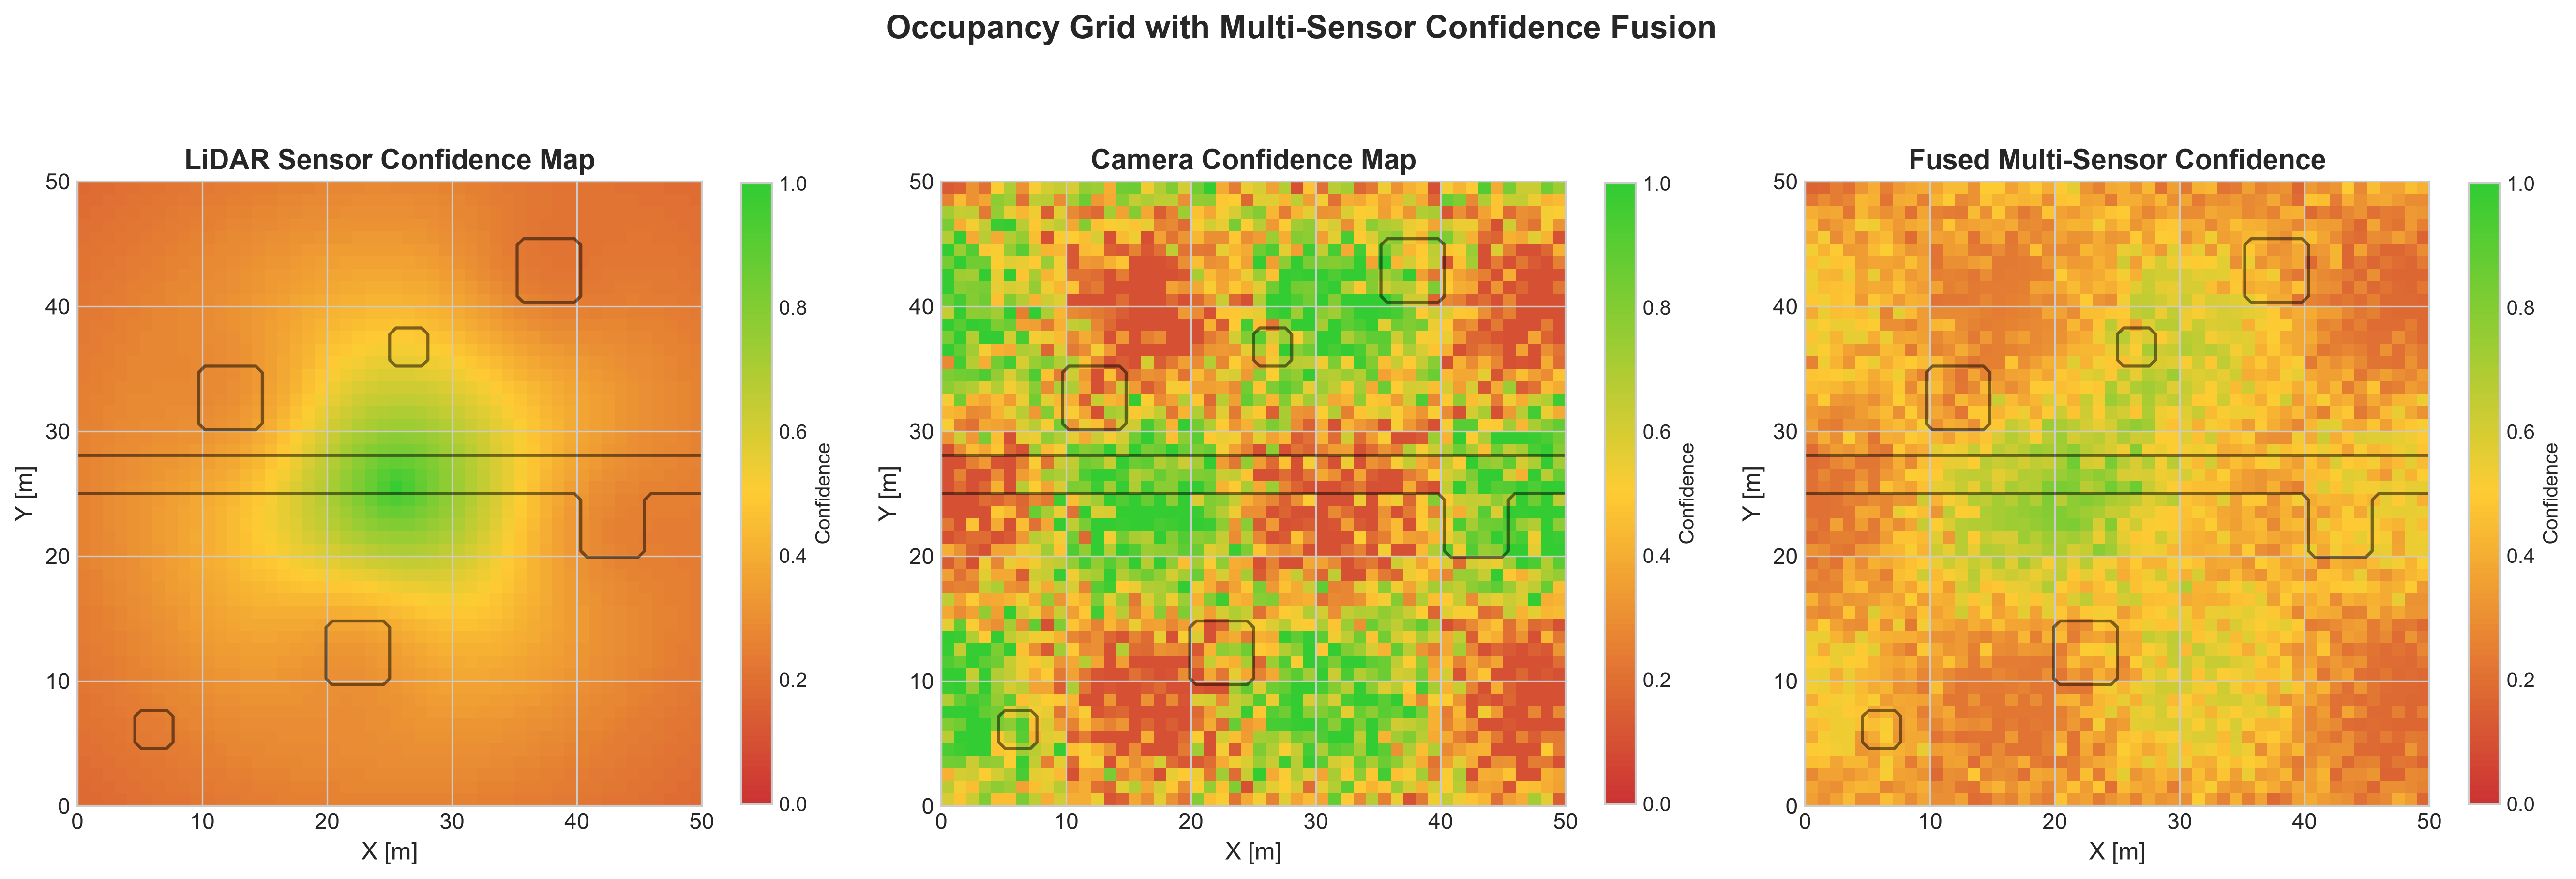
\includegraphics[width=\textwidth]{figures/fig_occupancy_confidence.png}
\caption{רשת תפוסה עם מיזוג ביטחון רב-חיישני. (Occupancy grid with multi-sensor confidence fusion: LiDAR confidence, camera confidence, and fused confidence with obstacle contours.)}
\label{fig:ch04_occupancy_confidence}
\end{figure*}

\subsection{אינטגרציית IMU ופרה-אינטגרציה}
\label{sec:ch04_imu_preint}

תורת הפרה-אינטגרציה של IMU \cite{Forster2017IMUPreint} מאפשרת ניסוח מדידות IMU כאילוצים יחסיים בין keyframes בפקטור גרף. הפרה-אינטגרציה מחשבת את השינוי היחסי בסיבוב, במהירות ובמיקום בין שני זמנים, תוך התחשבות בהטיות החיישן. השייר הפרה-אינטגרציה מוגדר כ:

\begin{equation}
\mathbf{r}_{\mathcal{I}_{ij}} = \begin{bmatrix}
2 \cdot \text{vec}\l$e$f$t( \mathbf{R}_{ij}^T \mathbf{R}_j^T \mathbf{R}_i \right)$$$ \\
\mathbf{R}_i^T (\mathbf{v}_j - \mathbf{v}_i - \mathbf{g} \Delta t_{ij}) - \Delta\mathbf{v}_{ij} \\
\mathbf{R}_i^T (\mathbf{p}_j - \mathbf{p}_i - \mathbf{v}_i \Delta t_{ij} - \frac{1}{2} \mathbf{g} \Delta t_{ij}^2) - \Delta\mathbf{p}_{ij}
\end{bmatrix}
\label{eq:ch04_imu_preint_residual}
\end{equation}

כאשר $\mathbf{R}_i, \mathbf{p}_i, \mathbf{v}_i$ הם הסיבוב, המיקום והמהירות בזמן $i$, $\mathbf{g}$ הוא וקטור הכבידה, ו-$\Delta\mathbf{R}_{ij}, \Delta\mathbf{v}_{ij}, \Delta\mathbf{p}_{ij}$ הם המדידות הפרה-אינטגרליות. שייר זה מאפשר שילוב מדידות IMU בפקטור הגרף ללא צורך באינטגרציה מחדש בכל איטרציה.

\subsection{סיכום}
\label{sec:ch04_summary}

פרק זה הציג את אלגוריתם ה-SLAM המרכזי של מערכת NavigatorCrew, המבוסס על אופטימיזציית פקטור גרף באמצעות iSAM2. האלגוריתם משלב שישה סוגי פקטורים: תנועה, LiDAR, מצלמה, סונאר, GPS ולולאות סגירה. מנגנון זיהוי הלולאות מבוסס DBoW2 עם אימות גאומטרי PnP+RANSAC מאפשר תיקון סחיפה מצטברת. אומדן הטווח מבוסס הסונאר הביו-מימטי, המחקה נוירוני עיכוב-מתואם בעטלפים, מספק רזולוציית טווח של 0.86 סנטימטרים. ניתוח הסיבוכיות מראה כי האלגוריתם פועל בזמן אמת על פלטפורמות משובצות, עם 25 FPS על Jetson Orin NX. מנגנון גיזום ה-keyframes שומר על גודל חסום של פקטור הגרף, ומנגנון fluid relinearization מקטין את עלות האופטימיזציה ב-60\%.